%%%
% Plantilla de Presentación
% Modificación de una plantilla de Latex de LaTeXTemplates para adaptarla
% al castellano y a las necesidades de escribir informática y matemáticas.
%
% Editada por: Mario Román
%
% License:
% CC BY-NC-SA 3.0 (http://creativecommons.org/licenses/by-nc-sa/3.0/)
%%%

%%%%%%%%%%%%%%%%%%%%%%%%%%%%%%%%%%%%%%%%%
% Beamer Presentation
% LaTeX Template
% Version 1.0 (10/11/12)
%
% This template has been downloaded from:
% http://www.LaTeXTemplates.com
%
% License:
% CC BY-NC-SA 3.0 (http://creativecommons.org/licenses/by-nc-sa/3.0/)
%
%%%%%%%%%%%%%%%%%%%%%%%%%%%%%%%%%%%%%%%%%

%----------------------------------------------------------------------------------------
%	PAQUETES Y CONFIGURACIÓN DEL DOCUMENTO
%----------------------------------------------------------------------------------------

\documentclass[8pt]{beamer}
%\geometry{paperwidth=140mm,paperheight=105mm}

%% Configuración de la presentación
\mode<presentation> {
  %%% Selección de estilo
  % The Beamer class comes with a number of default slide themes
  % which change the colors and layouts of slides. Below this is a list
  % of all the themes, uncomment each in turn to see what they look like.

  %\usetheme{default}
  %\usetheme{AnnArbor}
  %\usetheme{Antibes}
  %\usetheme{Bergen}
  %\usetheme{Berkeley}
  %\usetheme{Berlin}
  %\usetheme{Boadilla}
  %\usetheme{CambridgeUS}
  %\usetheme{Copenhagen}
  %\usetheme{Darmstadt}
  \usetheme[compress]{Dresden}
  %\usetheme{Frankfurt}
  %\usetheme{Goettingen}
  %\usetheme{Hannover}
  %\usetheme{Ilmenau}
  %\usetheme{JuanLesPins}
  %\usetheme{Luebeck}
  %\usetheme{Madrid}
  %\usetheme{Malmoe}
  %\usetheme{Marburg}
  %\usetheme{Montpellier}
  %\usetheme{PaloAlto}
  %\usetheme{Pittsburgh}
  %\usetheme{Rochester}
  %\usetheme{Singapore}
  %\usetheme{Szeged}
  %\usetheme{Warsaw}

  %% Selección de color
  % As well as themes, the Beamer class has a number of color themes
  % for any slide theme. Uncomment each of these in turn to see how it
  % changes the colors of your current slide theme.

  %\usecolortheme{albatross}
  %\usecolortheme{beaver}
  %\usecolortheme{beetle}
  %\usecolortheme{crane}
  %\usecolortheme{dolphin}
  %\usecolortheme{dove}
  %\usecolortheme{fly}
  \usecolortheme{lily}
  %\usecolortheme{orchid}
  %\usecolortheme{rose}
  %\usecolortheme{seagull}
  %\usecolortheme{seahorse}
  %\usecolortheme{whale}
  %\usecolortheme{wolverine}

  %% Configuración del pie de línea
  %\setbeamertemplate{footline} % To remove the footer line in all slides uncomment this line
  %\setbeamertemplate{footline}[page number] % To replace the footer line in all slides with a simple slide count uncomment this line
  %\setbeamertemplate{navigation symbols}{} % To remove the navigation symbols from the bottom of all slides uncomment this line
}

\setbeamertemplate{section in toc}[sections numbered]
\setbeamertemplate{subsection in toc}[subsections numbered]

%% Fuentes de tamaño arbitrario
\usepackage{lmodern}

\usepackage{listings}
\lstset{language=C++,
                basicstyle=\ttfamily,
                keywordstyle=\color{blue}\ttfamily,
                stringstyle=\color{red}\ttfamily,
                commentstyle=\color{green}\ttfamily,
                morecomment=[l][\color{magenta}]{\#}
}

%% Gráficos
\usepackage{graphicx} % Allows including images
\usepackage{booktabs} % Allows the use of \toprule, \midrule and \bottomrule in tables

\newcommand{\hlink}[2]{{\color{blue}\href{#1}{#2}}}
%%% Castellano.
% noquoting: Permite uso de comillas no españolas.
% lcroman: Permite la enumeración con numerales romanos en minúscula.
% fontenc: Usa la fuente completa para que pueda copiarse correctamente del pdf.
\usepackage[spanish,es-noquoting,es-lcroman]{babel}
\usepackage[utf8]{inputenc}
\usepackage[T1]{fontenc}
\selectlanguage{spanish}

%% Justificación del texto
\usepackage{ragged2e}
\usepackage{etoolbox}
\addtobeamertemplate{block begin}{}{\justifying}
\apptocmd{\frame}{\justifying}{}{}
%\apptocmd{\column}{\justifying}{}{}


\usepackage{tikz}
\usetikzlibrary{arrows}

%----------------------------------------------------------------------------------------
%	TÍTULO
%----------------------------------------------------------------------------------------

\title[]{Procesos estocásticos: } % The short title appears at the bottom of every slide, the full title is only on the title page
\subtitle[]{Modelos de colas}

\author[Marta Andrés, Ignacio Cordón, Bartolomé Ortiz] % Your name
{\texorpdfstring{
      \centering
      Marta Andrés, Ignacio Cordón, Bartolomé Ortiz\\
      \href{http://www.github.com/ncordon/queue-theory}{@ncordon/queue-theory}
}{Marta Andrés, Ignacio Cordón, Bartolomé Ortiz}}

\institute[UGR] % Your institution as it will appear on the bottom of every slide, may be shorthand to save space
{
  Universidad de Granada \\ % Your institution for the title page
  \medskip
  %\textit{autor@ugr.correo.es} % Your email address
}
\date{\today} % Date, can be changed to a custom date

% \subtitle{Y a la programación funcional}   % Subtítulo
% \author[@pbaeyens \and @M42]    % Autores (tex.stackexchange.com/questions/63259)
% {\texorpdfstring{
%     \begin{columns}
%       \column{.45\linewidth}
%       \centering
%       Pablo Baeyens\\
%       \href{http://www.github.com/pbaeyens}{@pbaeyens}
%       \column{.45\linewidth}
%       \centering
%       Mario Román\\
%       \href{http://www.github.com/M42}{@M42}
%     \end{columns}
% }{Pablo Baeyens \and Mario Román}}
% \date{OSL 2015}

\usepackage{scalerel}
\newcommand*\bigcdot{\mathpalette\bigcdot@{.5}}

\DeclareMathOperator*{\Bigcdot}{\scalerel*{\cdot}{\bigodot}}

\begin{document}

%% Diapositiva de título.
\begin{frame}
\titlepage % Print the title page as the first slide
\end{frame}

%% Diapositiva de contenidos.
% Throughout your presentation, if you choose to use \section{} and \subsection{} commands,
% these will automatically be printed on this slide as an overview of your presentation
\begin{frame}
  \frametitle{Contenidos} % Table of contents slide, comment this block out to remove it
  \tableofcontents
\end{frame}



%----------------------------------------------------------------------------------------
%	PRESENTACIÓN
%----------------------------------------------------------------------------------------

  \section{Introducción}
  \subsection{Distribución exponencial}
  \begin{frame}\frametitle{Definiciones}
    \begin{block}{Distribución exponencial}
      \[X \sim exp(\lambda),\lambda > 0 \Leftrightarrow F(x) = \left\{\begin{array}{ll}
      1- e^{-\lambda x} ,& x\ge 0 \\
      0 ,& x\le 0
      \end{array}\right.\]
    \end{block}

    \begin{block}{Propiedad de Markov}
      $X \ge 0$ tiene la propiedad de Markov si:
      \[P[X \ge t+h \mid X \ge t] = P[X \ge h] \qquad \forall t,h \in \mathbb{R}_0^{+}\]
      Equivalentemente:
      \[P[X < t+h \mid X \ge t] = P[X < h] = P[ 0 \le X < h] \qquad \forall t,h \in \mathbb{R}_0^{+}\]
    \end{block}
  \end{frame}
  \begin{frame}\frametitle{Propiedades}
    \begin{enumerate}
    \item
      $X \sim exp(\lambda) \Rightarrow X$ tiene la propiedad de Markov
    \item
      $X\ge 0$ continua con la propiedad de Markov $\Rightarrow X \sim exp(\lambda)$
    \end{enumerate}
  \end{frame}


  \subsection{Procesos de Poisson}
  \begin{frame}\frametitle{Notación}
    \begin{block}{Notación $o$}
    Una función $f$ se dice $o(h)$ (formalmente $f\in o(h)$) y lo notamos $f=o(h)$ si se verifica:
    \[\lim_{h\rightarrow 0} \frac{f(h)}{h} = 0\]
    \end{block}
    \begin{block}{Linealidad}
      Dados $c_1, \ldots c_n \in \mathbb{R}$, $f_1, \ldots f_n \in o(h)$, entonces $\sum_{i=1}^{n} c_i f_i = o(h)$
    \end{block}
  \end{frame}

  \begin{frame}\frametitle{Procesos de conteo}
    Sea $\{N_t\}_{t\ge 0}$ proceso estocástico discreto. Se dice que es proceso de conteo si se verifica:
    \begin{enumerate}
    \item No negatividad: $N_t \in \mathbb{N}\cup\{0\}, \quad \forall t\ge 0$. Además: $N_0=0$
    \item Monotonía: $N_s \le N_t, \quad \forall s \le t$
    \end{enumerate}

    $N_t$ indica el número de eventos que han ocurrido en el intervalo $[0,t]$. Por tanto $N_t- N_s$, con $t\ge s$
    indica el número de eventos que han ocurrido en $]s,t]$.
  \end{frame}

  \begin{frame}\frametitle{Procesos de Poisson}
    Un proceso de conteo $\{N_t\}_{t\ge 0}$ se dice que es de Poisson de parámetro $\lambda > 0$ si se verifica:

    \begin{enumerate}
    \item El proceso tiene incrementos independientes: dados $0 \le t_1 < \ldots < t_n$, se verifica que
      las variables $N_{t_1}, N_{t_2} - N_{t_1}, \ldots, N_{t_n}- N_{t_{n-1}}$ son independientes. Esto es, el número de eventos
      que se producen en intervalos disjuntos es independiente.
    \item El proceso tiene incrementos estacionarios: $dist(N_{t+h} - N_t)$ es la misma para cualesquiera
      $t\ge 0, h\ge 0$.
    \item $P[N_h = 1] = \lambda h + o(h)$, es decir, la probabilidad de que ocurra un evento en un intervalo de
      tiempo de longitud $h$ es casi proporcional a $h$, salvo por un término despreciable en comparación con dicho $h$, para
      $h$ suficientemente pequeño.
    \item $P[N_h \ge 2] = o(h)$.
    \end{enumerate}

    Se deduce que:
    \[P[N_h = 0] = 1 - P[N_h=1] - P[N_h \ge 2] = 1 -\lambda h - o(h)\]
  \end{frame}

  \begin{frame}\frametitle{Propiedades}
    La mayoría de modelos de colas asumen una distribución exponencial para tiempos entre llegadas y tiempos 
de servicio, o equivalentemente una distribución de Poisson para frecuencias de llegada y servicio.

    \begin{enumerate}
    \item
      Sea $\{N_t\}_{t\ge 0}$ un proceso de Poisson de parámetro $\lambda > 0$. Entonces la variable aleatoria $Y_t = N_t - N_0 = N_t$ que
      describe el número de eventos en cualquier intervalo de longitud $t > 0$ tiene una distribución de Poisson de parámetro
      $\lambda t$:

      \[P[Y_t = k] = P[N_t = k] = e^{-\lambda t} \frac{(\lambda t)^k}{k!}, \quad k\ge 0\]

    \item
      Sea $\{N_t\}_{t\ge 0}$ proceso de conteo. Sea $\{t_n\}_{n\ge 1}$ sucesión real estrictamente creciente y positiva, 
      que representa los tiempos de eventos, es decir \[t_n = \min \{t \ge 0: N_t = n\}\]

      LLamando $\tau_1= t_1, \tau_{n+1} = t_{n+1} - t_{n}, \quad \forall n\in \mathbb{N}$ tiempos entre llegadas. Entonces equivalen:

      \begin{itemize}
      \item $\{N_t\}_{t\ge 0}$ es proceso de Poisson.
      \item Los tiempos entre llegadas $\{\tau_n\}$ son variables exponenciales i.i.d. de media $\frac{1}{\lambda}$, esto es,
        $\tau_n \sim exp(\lambda)$.
      \end{itemize}
    \item
      Sea $\{N_t\}_{t\ge 0}$ proceso de Poisson donde un evento ha tenido lugar en $[0,t]$. Entonces siendo $Y$ la variable
      describiendo el tiempo de ocurrencia de dicho evento en el intervalo $[0,t]$, se tiene $Y \sim U([0,t])$.

    \end{enumerate}
  \end{frame}

  \subsection{Procesos de nacimiento y muerte}
  \begin{frame}\frametitle{Procesos de nacimiento y muerte}
    %% El parámetro $\lambda$ de un proceso de Poisson $\{N_t\}_{t\ge 0}$ puede ser visto como una tasa de nacimiento, ya que la probabilidad
    %% de que ocurra un evento en un intervalo de longitud $h > 0$ es $P[N_h-N_0=1] = \lambda h e^{-\lambda h} = \lambda h + o(h)$.
    %% Cuando suponemos que el parámetro no es constante, sino que depende de $n$ (cantidad de eventos que se han producido hasta el momento), esto
    %% es $\lambda_n$, entonces la cantidad de nacimientos (eventos producidos) en un intervalo de longitud $h$ es $\lambda_n h + o(h)$. Si además
    %% establecemos que se pueden producir muertes con una tasa $\mu_n$, donde la probabilidad de que se produzca una muerte en un intervalo de longitud
    %% $h$ es $\mu_n h + o(h)$ tenemos un proceso de nacimiento y muerte.
    Sea una cadena de Markov $\{N_t\}_{t\ge 0}$ con espacio de estados $\mathbb{N}\cup \{0\}$, donde el espacio de estados representa el número de individuos
    de un sistema (población). Entonces $\{N_t\}_{t\ge 0}$ se dice proceso de nacimiento y muerte si existen tasas no negativas de nacimiento y muerte,
    $\{\lambda_n\}_{\mathbb{N}\cup \{0\}}$ y $\{\mu_n\}_{\mathbb{N}\cup \{0\}}$ y se verifica:
    \begin{enumerate}
    \item La población puede aumentar o decrecer únicamente de uno en uno.
    \item Si el sistema está en estado $n\ge 0$ entonces el tiempo hasta que el sistema está en estado $n+1 \ge 0$ es una variable aleatoria exponencial
      de paŕámetro $\lambda_n$.
    \item Si el sistema está en estado $n\ge 1$ entonces el tiempo hasta que el sistema está en estado $n-1 \ge 0$ es una variable aleatoria exponencial
      de paŕámetro $\mu_n$.
    \item Cualesquiera dos transiciones son independientes.
    \end{enumerate}
  \end{frame}

  \begin{frame}\frametitle{Cosas de Nacho}

  \end{frame}


  \section{El modelo de colas}
  \subsection{Definición}
  \begin{frame}\frametitle{Ilustración de las variables clave}
    \begin{figure}[h]
      \centering
      \begin{tikzpicture}
        \draw (20,5.5) rectangle (22,6);
        \node [above] at (21,5.5) {Servidor 1};
        \draw (20,4.5) rectangle (22,5);
        \node [above] at (21,4.5) {Servidor 2};
        \draw [dotted, ultra thick] (21,4.15) -- (21,3.85);
        \draw (20,3) rectangle (22,3.5);
        \node [above, blue] at (21,3) {Servidor $c$};

        \draw [fill] (19.5,5.75) circle [radius=0.1];
        \draw [fill=white] (19.5,4.75) circle [radius=0.1];
        \draw [fill] (19.5,3.25) circle [radius=0.1];
        \draw [dashed, blue] (19.25,3) rectangle (19.75,6);
        \node [below, blue] at (19.5,3) {$N_{S,t}$};

        \draw [latex-latex, blue] (19.25,6.5) -- (22,6.5);
        \draw [blue] (19.25,6) --(19.25,6.6);
        \draw [blue] (22,6) --(22,6.6);
        \node [above, blue] at (20.7,6.5) {$S$};

        \draw (22.15,6) -- (22.5,6) -- (22.5,3) -- (22.15,3);
        \draw [-latex] (22.5,4.5) -- (23.5,4.5);

        \draw (19,6) -- (18.65,6) -- (18.65,3) -- (19,3);
        \draw [-latex] (18,4.5) -- (18.65,4.5);
        \draw [fill] (18,4.5) circle [radius=0.1];
        \draw [fill] (17.6,4.5) circle [radius=0.1];
        \draw [dotted, ultra thick] (17,4.5) -- (17.3,4.5);
        \draw [fill] (16.7,4.5) circle [radius=0.1];
        \draw (16,4.5) -- (16.6,4.5);
        \draw [blue] (16.6,4.3) -- (16.6,4.1) -- (18.1,4.1) -- (18.1,4.3);
        \node [below, blue] at (17.35,4.1) {$N_{Q,t}$};

        \draw [latex-latex, blue] (16.05,5) -- (18.6,5);
        \node [above, blue] at (17.34,5) {$Q$};

        \draw (16,2) rectangle (23,7.5);
        \node [above] at (19.5,7.5) {Sistema de encolado};

        \draw [-latex] (13.6,4.5) -- (16,4.5);
        \draw [fill] (14.25,4.5) circle [radius=0.1];
        \draw [fill] (15.25,4.5) circle [radius=0.1];

        \draw [latex-latex, blue] (14.25,5) -- (15.25,5);
        \draw [blue] (14.25,4.65) --(14.25,5.1);
        \draw [blue] (15.25,4.65) --(15.25,5.1);
        \node [above, blue] at (14.75,5) {$\tau$};
      \end{tikzpicture}
    \end{figure}

  \end{frame}
  \begin{frame}\frametitle{Definición de las variables clave}
    \begin{itemize}
    \item [$c$]
      Número (fijo) de servidores o canales en el sistema, $c\in \mathbb{N} \cup \{+\infty\}$
    \item [$\tau$]
      Variable aleatoria que describe el tiempo entre llegadas (de clientes).
    \item [$S$]
      Variable aleatoria que describe el tiempo de servicio.
    \item [$Q$]
      Variable aleatoria que describe el tiempo que espera un cliente en la cola.
    \item [$N_{S,t}$]
      Variable aleatoria que describe el número de clientes que están siendo servidos en el instante $t$.
    \item [$N_{Q,t}$]
      Variable aleatoria que describe el número de clientes en la cola (esperando a ser servidos) en el instante $t$.
    \end{itemize}
  \end{frame}

  \begin{frame}\frametitle{Otras variables relevantes}
    \begin{itemize}
    \item [$\lambda$]
      Frecuencia o tasa media de llegadas de clientes al sistema: $\lambda = 1/E[\tau]$.
    \item [$\mu$]
      Frecuencia o tasa media de servicio de los servidores del sistema: $\mu = 1/E[S]$.
    \item [$\rho$]
      Aprovechamiento de los servidores, esto es, la proporción de tiempo que los servidores están trabajando: $\rho = \frac{\lambda}{c\mu}$.
    \item [$W_S$]
      Tiempo medio que está siendo servido un cliente: $W_S  = E[S]$.
    \item [$W_Q$]
      Tiempo medio que está un cliente en la cola: $W_Q = E[Q]$.
    \item [$W$]
      Tiempo de espera. Variable aleatoria que describe el tiempo total que un cliente está en el sistema
      de encolado: $W = Q+S$.
    \item [$W_W$]
      Tiempo medio (de espera) que está un cliente en el sistema: $W_W = E[W]$.
    \item [$N_S$]
      Variable aleatoria que describe el número de clientes siendo servidos con el sistema en equilibrio: $N_S = \lim_{t \rightarrow \infty} N_{s,t}$.
    \item [$L_S$]
      Número medio de clientes siendo servidos con el sistema en equilibrio: \\ $L_S = E[N_S]$.
    \item [$N_Q$]
      Variable aleatoria que describe el número de clientes en la cola con el sistema en equilibrio: $N_Q = \lim_{t \rightarrow \infty} N_{Q,t}$.
    \item [$L_Q$]
      Número medio de clientes en la cola con el sistema en equilibro: $L_Q = E[N_Q]$.
    \item [$N_t$]
      Variable aleatoria que describe el número de clientes en el sistema en el instante $t$: $N_t = N_{Q,t} + N_{S,t}$.
    \item [$N$]
      Variable aleatoria que describe el número de clientes en el sistema con el sistema en equilibrio $N = N_Q + N_S$.
    \item [$L$]
      Número medio de clientes en el sistema en equilibrio: $L = E[N]$.
    \item [$P_n(t)$]
      Probabilidad de que haya $n$ clientes en el sistema en el instante $t$: es la función masa de probabilidad de $N_t$.
    \item [$p_n$]
      Probabilidad de que haya $n$ clientes en el sistema con el sistema en equilibrio: $p_n = \lim_{t \rightarrow \infty} P_n(t)$ es la función masa de probabilidad de $N$.
    \end{itemize}
  \end{frame}

  \subsection{Características}
  \begin{frame}\frametitle{Modelo de llegadas}
    \begin{block}{Definición}
    LLamamos modelo de llegadas a la distribución $A(t)$ de los tiempos entre llegadas $\{\tau_n\}$.
    \end{block}
    \begin{block}{Definición}

    El modelo de llegadas se dice:
 
    \begin{enumerate}
    \item Estacionario, cuando no depende del tiempo (por ejemplo cuando existe una distribución límite y hablamos
      del modelo de llegadas de dicha distribución límite).
    \item Transitorio, en caso opuesto.
    \end{enumerate}
    \end{block}
    \begin{block}{Definición}

      Para un modelo de llegadas, sea $A(t)$ función de distribución de los $\tau_n$.
      El modelo de llegadas se dice:

      \begin{enumerate}
      \item Aleatorio o de Poisson: si $A(t) = 1 - e^{-\lambda t}$.
      \item Determinístico: si $A(t) = \left\{\begin{array}{ll}
        0 & t<s \\
        1 & t\ge s
      \end{array}\right.$ con $s$ fijo.

      \end{enumerate}
    \end{block}
  \end{frame}
  \begin{frame}\frametitle{Modelo de servicio}
    Se pueden efectuar unas definiciones análogas para modelo determinístico, aleatorio y régimen estacionario y transitorio
    de servicio a las que se han hecho con el modelo de llegadas.

    \begin{block}{Caso particular, modelo de Poisson de servicio}

      Supongamos que el modelo de colas tiene $k$ servidores o canales para atender peticiones, y el tiempo que 
      tarda cada uno en atender una petición $T_i, i=1,\ldots k$ sigue una distribución exponencial de parámetro $\bar{\mu}$.
      Entonces el tiempo hasta terminar de atender una petición es $T = min\{T_1, \ldots T_n\}$. Por propiedades de la
      distribución exponencial deducimos que $T$ sigue una distribución exponencial de parámetro $\mu = n \bar{\mu}$
      
      La función de distribución de $W_S$ por tanto sería $W_S[t] = P[S\le t] = 1 - e^{-\mu t}$.

    \end{block}


  \end{frame}
  \begin{frame}\frametitle{Capacidad del sistema}
    Sea $S\subseteq \mathbb{N}$ el menor espacio de estados sobre el que está definido el proceso estocástico $\{N_{Q,t}\}_{t\ge 0}$ . 
    Se llama capacidad al tamaño máximo de la cola de peticiones, esto es $M = \max S \in \mathbb{N} \cup \{+\infty\}$. 
    Por tanto no puede tenerse que en ningún tiempo $N_{Q,t}$ tome un valor mayor que $M$, y si llegara una
    petición cuando la cola tiene tamaño $M$, se rechazaría dicha petición.
  \end{frame}
  \begin{frame}\frametitle{Comportamiento de los clientes}
    Podemos considerar que los clientes que llegan a la cola pueden efectuar:

    \begin{itemize}
    \item Oposición: una petición se retira en la llegada (por ejemplo en casos en los que la cola sea muy larga
      y el cliente se abstenga de entrar).
    \item Retirada: la petición entra a la cola, pero tras un tiempo de espera, la deja.
    \item Recolocación: si hay varias colas paralelas, los clientes se pueden cambiar de una cola a otra.
    \item Priorización: algunos clientes pueden tener mayor prioridad que otros al ser servidos.
    \end{itemize}

  \end{frame}
  \begin{frame}\frametitle{Disciplina de la cola}
    Se pueden tener distintas formas de elegir de la cola el siguiente cliente a ser servido. Consideramos las siguientes estrategias:
    \begin{itemize}
    \item FIFO (First in, first out): es la cola tradicional, en la que el cliente que lleva más tiempo esperando en la cola es el siguiente en ser servido.
    \item LIFO (Last in, first out): el cliente que lleva menos tiempo esperando en la cola es el siguiente en ser servido.
    \item SIRO (Service in random order): se escoge un cliente al azar de entre todos los de la cola, con probabilidad uniforme.
    \item PRI (Priority  service): los clientes tienen asignado un nivel de prioridad y se elige el cliente con mayor prioridad de la cola. En caso de haber varios con la misma probabilidad, se usa alguna de las disciplinas anteriores para elegir entre ellos.
    \end{itemize}

  \end{frame}

  \subsection{Notación de Kendall}
  \begin{frame}\frametitle{Notación de Kendall}
    \begin{exampleblock}{$$A/B/c/K/m/Z$$}
    \end{exampleblock}
    \begin{itemize}
    \item $A$ y $B$: describen $\tau$ y $S$ con los símbolos:
      \begin{itemize}
      \item [$G$]
        General: sólo se asume que $\tau_n$ o $S_n$ son independientes
      \item [$D$]
        Determínistica: $\tau$ es constante
      \item [$M$]
        De Markov: $\tau \sim exp(\lambda)$
        %% Estas dos no aparecen en en el apartado 2.1.1, ponerlas?
        %% \item [$E_k$] Erlang-k
        %% \item [$H_k$] k-stage hyperexponential
      \end{itemize}
    \item $c$: número de servidores
    \item $K$: capacidad máxima del sistema
    \item $m$: tamaño de la población
    \item $Z$: la disciplina de la cola (FIFO, LIFO, etc.)
    \end{itemize}

    Notación acortada (suponemos $K=\infty,m=\infty,Z=FIFO$):
    \begin{exampleblock}{$$A/B/c$$}
    \end{exampleblock}
  \end{frame}

  \subsection{Medidas de efectividad}
  \begin{frame}\frametitle{Medidas de efectividad}
    \begin{itemize}
    \item Aprovechamiento de los servidores: $\rho = \frac{\lambda}{c\mu}$
    \item Intensidad de tráfico: $a= W_S/E[\tau]$
    \item Tiempo medio de un cliente en el sistema: $W_W$
    \item Tiempo medio de un cliente en la cola: $W_Q$
    \item Percentil 90 del tiempo total en el sistema $W_W$: $\pi_{W} \lbrack 90 \rbrack$
    \item Percentil 90 del tiempo de espera en la cola $W_Q$: $\pi_{W} \lbrack 90 \rbrack$
    \item Número medio de clientes en el sistema: $L$
    \item Número medio de clientes en la cola: $L_Q$
    \item Probabilidad de que haya $n$ clientes en el sistema: $p_n$
    \end{itemize}
  \end{frame}

  \section{Leyes de Little}
  \begin{frame}\frametitle{Notación}
    Para $n \geq 1$, llamemos al cliente $n$-ésimo, el cual llega en el instante $t_n$, nombremos $W_n$ al tiempo 
    de espera del cliente con lo cual es inmediato deducir, que nuestro cliente abandonará la cola en el instante
    $t_n + W_n$, donde $0 = t_0 \leq t_1 \leq t_2 \leq... $.
    
    Es inmediato tambien que podemos definir una función indicadora que refleje si el $c_n$ está o no en el
    sistema:
    
    Indicador: $I_n(t) = \left\{\begin{array}{cc}
    1, & t_n \leq t <t_n + W_n\\
    0, & \textrm{en otro caso}
    \end{array}\right.$, de donde  $\int_{0}^{\infty} I_n(t)dt=W_n$.
    
    Sea $\Delta(t) = max \{i: t_n \leq t\}$ el número de llegadas en tiempo t. El número de clientes en el sistema
    viene dado por:
    
    \[N_t = \sum_{i=1}^{\Delta(t)} I_n(t)\]
  \end{frame}

  \begin{frame}
    A partir del tiempo de llegada ${t_n}$ y del tiempo de servicio ${W i}$ del cliente $i$-ésimo, podemos 
    construir ${N_t}$ paratodo $t$. Visualmente podemos entender de forma sencilla estos conceptos si trazamos 
    ${\Delta (t)}$ como una función escalonada y mostramos un tiempo de espera del cliente.

    \begin{figure}[H]
      \begin{center}
        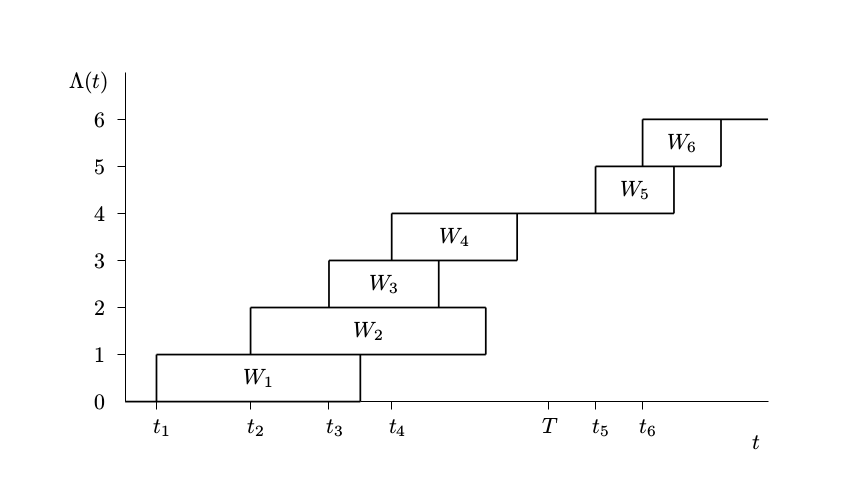
\includegraphics[width=0.9\textwidth]{./imgs/fig1.png}
      \end{center}
    \end{figure}

  \end{frame}

  \begin{frame}
    A su vez podemos representar $N_t$ como una función escalonada (cuya información será obviamente menor que la primera figura) 
    representando únicamente el número de personas en el sistema.

    \begin{figure}[H]
      \begin{center}
        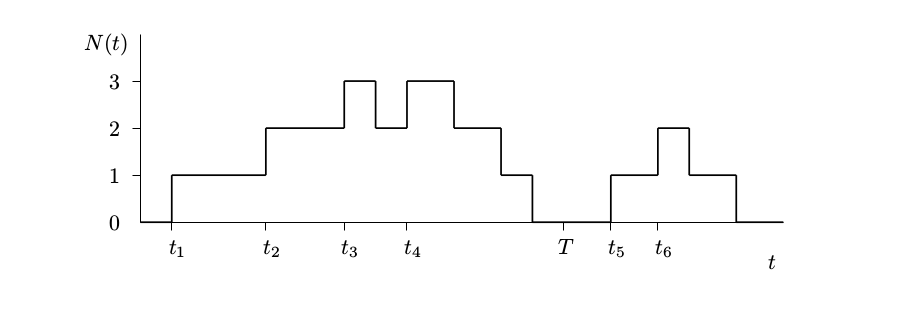
\includegraphics[width=\textwidth]{./imgs/fig2.png}
      \end{center}
    \end{figure}
  \end{frame}
  \begin{frame}\frametitle{Cosas de Bart}
  \end{frame}

  \begin{frame}\frametitle{Teorema de Little}
    Si los límites $\lambda$ y $W_W$ existen y son finitos, entonces $L$ existe y es finito, donde 
    \[L = \lambda W_W\]
  \end{frame}
\section{Modelos particulares}

  \subsection{Modelo D/D/1}
  \begin{frame}\frametitle{Caso $\lambda > \mu$}
    Intuitivamente, la cola será inestable y no podrá servir todas las peticiones. 

    Se tiene $a > 1$, $\rho > 1$.

    \begin{block}{Proposición}
      Notando $Q_n$ al tiempo de espera del $n$ ésimo cliente, tenemos que \[Q_1 = 0, \qquad Q_n = \left(\frac{1}{\mu} - \frac{1}{\lambda}\right)n, \quad \forall n\ge 2\]
    \end{block}

    \begin{block}{Corolario}
      El tiempo de espera total para el $n$ ésimo cliente es:
 
      \[W_1 = \frac{1}{\mu}, \qquad W_n = \left(\frac{1}{\mu} - \frac{1}{\lambda}\right)^n + \frac{1}{\mu} \quad n\in \mathbb{N}\]
    \end{block}

    \begin{block}{Proposición}
      En un instante $t$ el número de clientes en el sistema será: 
      \[N_t = \left\{\begin{array}{lcc}
      0, && t < \frac{1}{\lambda}\\
      \lfloor t\lambda \rfloor - \left\lfloor\left(t-\frac{1}{\lambda}\right)\mu\right\rfloor, && \text{otro caso}
      \end{array}\right.\]
    \end{block}

  \end{frame}

  \begin{frame}\frametitle{Caso $\lambda \le \mu$}
    Se tiene $a < 1$, $\rho < 1$.

    \begin{block}{Proposición}
Se tiene $\forall n\in \mathbb{N}$:

\begin{align*}
Q_n = 0\\
W_n = \frac{1}{\mu}
\end{align*}
    \end{block}

    \begin{block}{Corolario}
 El tiempo de espera total para el $n$ ésimo cliente es únicamente el tiempo en ser servido.
    \end{block}

    \begin{block}{Proposición}
 En un instante $t$ el número de clientes en el sistema será: 
 \[N_t = \left\{\begin{array}{lcc}
          0, && t < \frac{1}{\lambda}\\
          0, && t \ge \frac{1}{\lambda}, t \in \left]\frac{n-1}{\lambda} + \frac{1}{\mu}, \frac{n-1}{\lambda} + \frac{1}{\lambda}\right[\\
          1, && \text{otro caso}
         \end{array}\right.\]
    \end{block}
  \end{frame}

  \subsection{Modelo M/M/1}
  \begin{frame}\frametitle{Chino mandarín}
    
  \end{frame}

  \section{Ejemplos}
  \begin{frame}\frametitle{Paradoja del tiempo de espera}
    El autobús pasa cada $\alpha$ minutos por la parada, y llegamos en un momento aleatorio. ¿Cuánto tiempo esperamos que tarde en llegar el autobús?

    Intuición:  $\frac{\alpha}{2} \Rightarrow$  FALSO!

    Respuesta correcta: depende de la varianza del tiempo entre llegadas
    \begin{itemize}
    \item Varianza 0: $\frac{\alpha}{2}$
    \item Varianza infinita: tiempo infinito
    \end{itemize}
  \end{frame}

%% Bibliografía
\section {Referencias}
\begin{frame}
\frametitle{Referencias}
\footnotesize{
  \begin{thebibliography}{99} % Beamer does not support BibTeX so references must be inserted manually as below
    \bibitem[Allen, 1990]{allen} Arnold O.Allen
      \newblock Probability, Statistics and Queueing Theory with Computer Science Applications\\
      \newblock \emph{Academic Press}

    \bibitem[Gross, 2008]{gross} Donald Gross, John F.Shortle, James M.Thompson, Carl M.Harris
      \newblock Fundamentals of Queueing Theory\\
      \newblock \emph{Wiley}

    \bibitem[Gunavathi, 2010]{gunavathi} P.Kandasamy, K.Thilagavathi, K.Gunavathi
      \newblock Probability and Queueing Theory (2010)\\
      \newblock \emph{S. Chand \& Company}

    \bibitem[Wolff, 2011]{wolff} Ronald W. Wolff
      \newblock Little's law and Related Results\\
      \newblock \emph{University of California at Berkeley}

  \end{thebibliography}
}
\end{frame}
\end{document}
